\section{The quadratic relation in general}

    In this section we show that for any character $\chi=\chi_0\otimes\ldots\otimes\chi_n$ of $T(\cO)\subset\GL_{n+1}(F)$ and $s\in S_{\chi,\aff}$, the proof of the quadratic relation for $\varphi_s=q^{(1-l(s))/2}[IsI]_{\check{\chi}}$ can be deduced from the particular case proven in the previous section. Let $\Phi$ be the root system for $\GL_{n+1}$ with simple roots $\Pi=\{\alpha_1,\ldots,\alpha_n\}$. For each $w\in\widetilde{W}$, let 
    $$\widetilde{\Delta}(w)=\{\text{hyperplanes }P\ |\ P\text{ separates }\mathcal{D}_0\text{ and }w\mathcal{D}_0\}.$$
    Recall from Iwahori-Matsumoto that $l(w)=|\widetilde{\Delta}(w)|$ for all $w\in\widetilde{W}$.

    \begin{lemma}\label{lem_w1}
        Let $\alpha=\sum_{k=i}^{j}\alpha_k\in\Phi^+$ for some $i\leq j$. Then
        \begin{align*}
            \widetilde{\Delta}(w_\alpha(1))&=\{P_{\beta,0}\ |\ \beta\in\Phi^+\cap w_\alpha^{-1}\Phi^-\}\\
            %=\{P_{\alpha,0}\}\cup\{P_{\beta,0}:\beta\in\Phi^+,\langle\beta,\calpha\rangle=1\text{ and }\alpha-\beta\in\Phi^+\}\\
            &=\{P_{\alpha_i,0},P_{\alpha_i+\alpha_{i+1},0},\ldots,P_{\alpha,0},\ldots,P_{\alpha_{j-1}+\alpha_j,0},P_{\alpha_j,0}\}.
        \end{align*}
    \end{lemma}

    \begin{proof}
        Let $x\in\mathcal{D}_0$ and let $\beta\in\Phi^+$. Then
        \begin{equation*}
            \langle\beta,w_\alpha(1)(x)\rangle=\langle\beta,x\rangle-\langle\alpha,x\rangle\langle\beta,\calpha\rangle=\langle w_\alpha(\beta),x\rangle\in
            \begin{cases}
                (0,1) &\text{ if } w_\alpha(\beta)\in\Phi^+,\\
                (-1,0) &\text{ if } w_\alpha(\beta)\in\Phi^-.
            \end{cases}
        \end{equation*}
        Hence, $P\in\widetilde{\Delta}(w)$ if and only if $P=P_{\beta,0}$ for some $\beta\in\Phi^+\cap w_\alpha^{-1}\Phi^{-1}$. Since $w_\alpha(\beta)=\beta-\langle\beta,\calpha\rangle\alpha$, it follows that $\beta\in\Phi^+\cap w_\alpha^{-1}\Phi^-$ if and only if $\beta=\alpha$ or $\langle\beta,\calpha\rangle=1$ and $\alpha-\beta\in\Phi^+$.
        
        If $\alpha=\alpha_i+\cdots+\alpha_j$ for some $j\geq i$, then a standard calculation shows that $\beta\in\Phi^+$ satisfies the above conditions if and only if $\beta=\alpha_i+\cdots+\alpha_k$ for some $k\leq j$ or $\beta=\alpha_k+\cdots+\alpha_j$ for some $k\geq i$. This concludes the proof.
    \end{proof}

    \begin{lemma}\label{lem_wvarpi}
        Let $\alpha=\sum_{k=i}^{j}\alpha_k\in\Phi^+$ for some $i\leq j$. Then
        \begin{align*}
            \widetilde{\Delta}(w_\alpha(\varpi^{-1}))&=\{P_{\alpha_1+\cdots+\alpha_{i-1},0},\ldots,P_{\alpha_{i-1},0},P_{\alpha_{j+1},0},\ldots,P_{\alpha_{j+1}+\cdots+\alpha_{n},0}\}\\
            %=\{P_{\alpha,0}\}\cup\{P_{\beta,0}:\beta\in\Phi^+,\langle\beta,\calpha\rangle=1\text{ and }\alpha-\beta\in\Phi^+\}\\
            &\cup\{P_{\alpha_1+\cdots+\alpha_j,1},\ldots,P_{\alpha_i+\cdots+\alpha_{j},1},\ldots,P_{\alpha_i+\cdots+\alpha_n,1}\}.
        \end{align*}
    \end{lemma}

    \begin{proof}
        As in the previous proof, let $x\in\mathcal{D}_0$ and let $\beta\in\Phi^+$. Then,
        \begin{align*}
            \langle\beta,w_\alpha(\varpi^{-1})(x)\rangle=\langle\beta,x\rangle-\langle\alpha,x\rangle\langle\beta,\calpha\rangle+\langle\beta,\calpha\rangle=\langle w_\alpha(\beta),x\rangle+\langle\beta,\calpha\rangle\\
            \in
            \begin{cases}
                (1,2) &\text{ if } \beta=\alpha \text{, or } \langle\beta,\calpha\rangle=1 \text{ and } w_\alpha(\beta)\in\Phi^+,\\
                (0,1) &\text{ if } \langle\beta,\calpha\rangle=0 \text{, or }\langle\beta,\calpha\rangle=1 \text{ and }w_\alpha(\beta)\in\Phi^-,\\
                (-1,0) &\text{ if } \langle\beta,\calpha\rangle=-1.
            \end{cases}
        \end{align*}
    
        Thus,
        \begin{equation*}
            \widetilde{\Delta}(w_\alpha(\varpi^{-1}))=\{P_{\alpha,1}\}\cup\{P_{\beta,1}\ |\ \beta\in\Phi^+,\langle\beta,\calpha\rangle=1 \text{ and }w_\alpha(\beta)\in\Phi^+\}\cup\{P_{\beta,0}\ |\ \beta\in\Phi^+\text{ and }\langle\beta,\calpha\rangle=-1\}.
        \end{equation*}
        If $\alpha=\alpha_i+\cdots+\alpha_j$, then further calculations show that $\beta\in\Phi^+$ satisfies $\langle\beta,\calpha\rangle=1$ with $w_\alpha(\beta)=\beta-\alpha\in\Phi^+$ if and only if $\beta=\alpha_k+\cdots+\alpha_j$ for some $k<i$ or $\beta=\alpha_i+\cdots+\alpha_k$ for some $k>j$. Similarly, one can show that $\beta\in\Phi^+$ satisfies $\langle\beta,\calpha\rangle=-1$ if and only if $\beta=\alpha_k+\cdots+\alpha_{i-1}$ for some $k\leq i-1$ or $\beta=\alpha_{j+1}+\cdots+\alpha_k$ for some $k\geq j+1$.
    \end{proof}


    \begin{cor}\label{cor_lengthsum}
        For any $\alpha\in\Phi^+$, we have that 
        $$l(w_\alpha(1))+l(w_\alpha(\varpi^{-1}))=\sum_{\beta\in\Phi^+}|\langle\beta,\calpha\rangle|=2n$$
    \end{cor}
    \begin{proof}
        The first equality is an immediate consequence of $l(w)=\widetilde{\Delta}(w)$ together with Lemmas \ref{lem_w1} and \ref{lem_wvarpi}. Indeed, if $\langle\beta,\calpha\rangle=0$ then no hyperplane arising from $\beta$ lies in $\widetilde{\Delta}(w_\alpha(1))\cup\widetilde{\Delta}(w_\alpha(\varpi^{-1}))$; if $\langle\beta,\calpha\rangle=\pm1$, then exactly one plane arising from $\beta$ lies $\widetilde{\Delta}(w_\alpha(1))\cup\widetilde{\Delta}(w_\alpha(\varpi^{-1}))$; finally, $P_{\alpha,0}\in \widetilde{\Delta}(w_\alpha(1))$ and $P_{\alpha,1}\in \widetilde{\Delta}(w_\alpha(\varpi^{-1}))$.

        The second part of the lemma is a direct computation: if $\alpha=\alpha_i\cdots\alpha_j$, then there are 
        \begin{itemize}
            \item $j$ roots in $\Phi^+$ of the form $\alpha_k+\cdots+\alpha_j$ for $k\leq j$,
            \item $n+1-i$ roots in $\Phi^+$ of the form $\alpha_i+\cdots+\alpha_k$ for $k\geq i$,
            \item $i-1$ roots in $\Phi^+$ of the form $\alpha_k+\cdots+\alpha_{i-1}$ for $k\leq i-1$,
            \item $n+1-(j+1)$ roots in $\Phi^+$ of the form $\alpha_{j+1}+\cdots+\alpha_k$ for $k\geq j+1$.
        \end{itemize}
        Giving a total of $2n$ roots, each of which contributes once towards $\sum_{\beta\in\Phi^+}|\langle\beta,\calpha\rangle|$, as desired.
    \end{proof}

    \subsection{The diagram associated to a character}
    Having established the preliminary lemmas, we now consider a depth zero character $\chi=\chi_0\otimes\cdots\otimes\chi_n$ of $T(\cO)\subset\GL_{n+1}(F)$, where each $\chi_i$ is a depth-zero character of $\cO^\times$. The character $\chi$ induces a partition $\mathcal{P}_\chi$ of the set $\{0,1,\ldots,n\}$ according to which two elements $i,j\in\{0,1,\ldots,n\}$ are related if and only if $\chi_i=\chi_j$ as characters of $\cO^\times$. 
    
    %Denote by $\mathfrak{D}_{n}$ the affine Dynkin diagram of type $A_n$ (a regular polygon whose vertices are labelled $\alpha_0,\alpha_1,\ldots,\alpha_n$ counterclockwise), with the \textit{distinguished} vertex $\alpha_0$.

    \begin{definition}
        Let $\chi$ be a depth-zero character of $T(\cO)\subset\GL_{n+1}(F)$ giving rise to a partition $\mathcal{P}_\chi$ of $\{0,1,\ldots,n\}$ of size $r$. Then the diagram $\mathfrak{D}_\chi$ associated to $\chi$ is a regular $(n+1)$-gon whose vertices are labelled $\{0,1,\ldots,n\}$ counterclockwise and have been painted in $r$ different colors according to the partition $\mathcal{P}_\chi$, and having a distinguished edge $e=\{0,n\}$.
    \end{definition}


    \begin{example}
        In the previous section we considered the family of characters $\chi=\chi_0\otimes\cdots\otimes\chi_n$ such that $\chi_0=\chi_n$ and all the remaining characters are distinct. Then $\mathcal{P}_\chi=\{\{0,n\},\{1\},\ldots,\{n-1\}\}$ has size $n$, and Figure \ref{fig_diagn4} shows the diagram with $n=4$.
        \begin{figure}[h]
            \begin{center}
                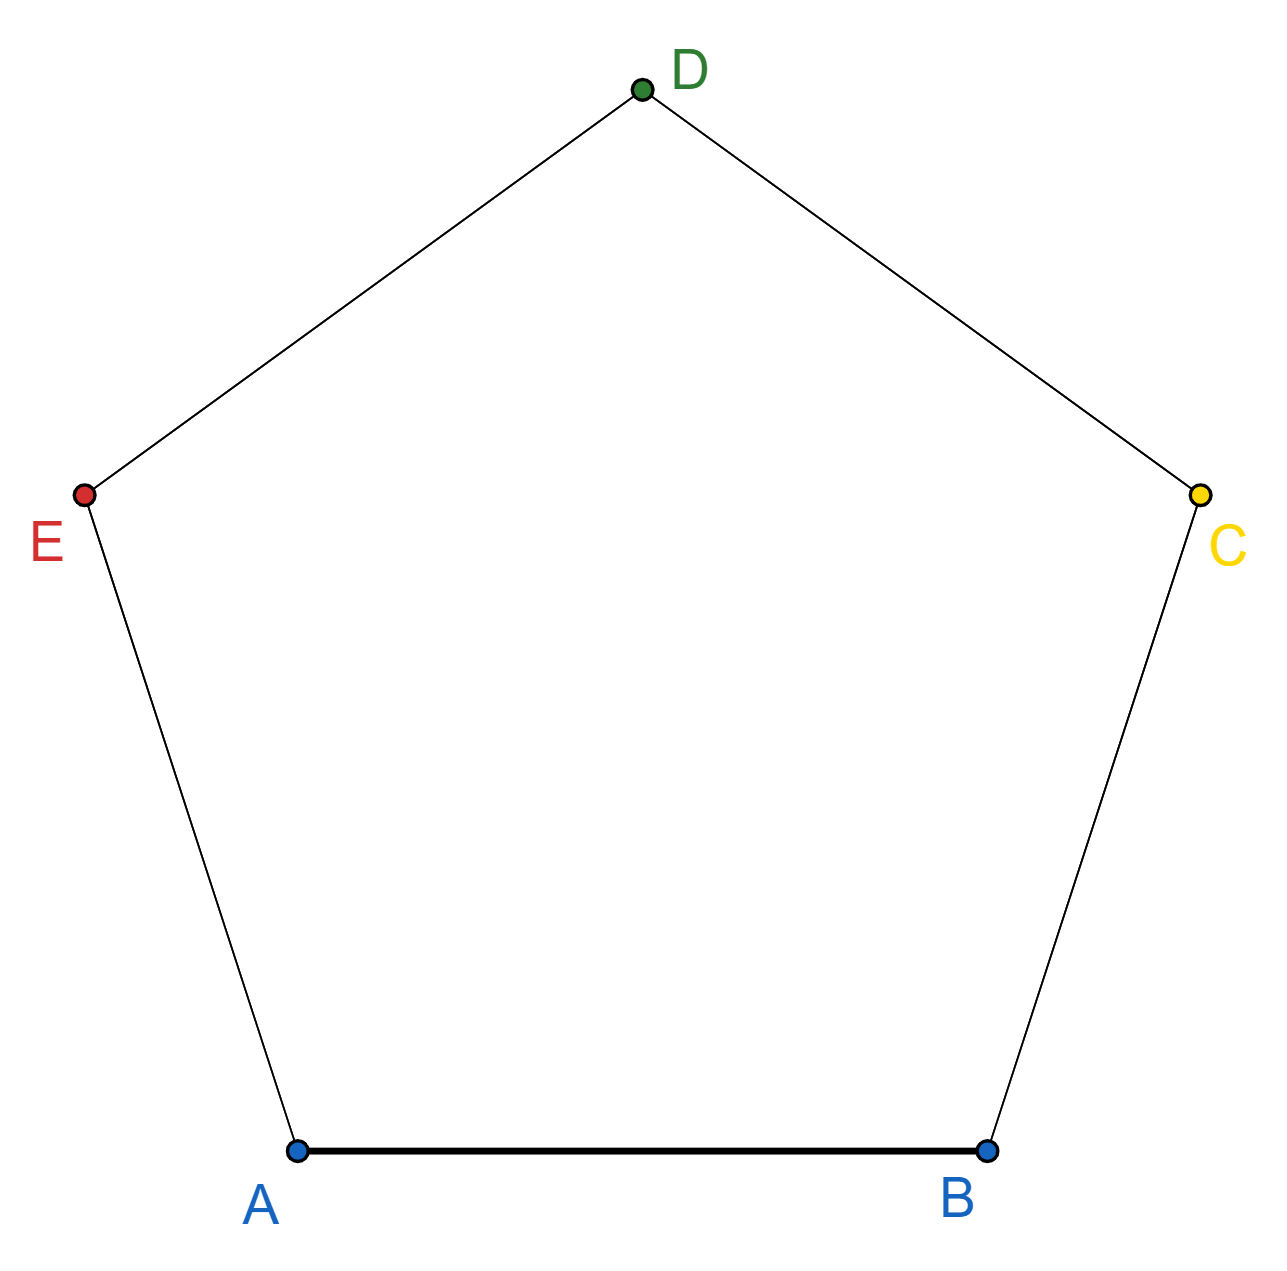
\includegraphics[scale=0.8]{geogebra-export.png}
                \caption{Diagram for $\mathcal{P}_\chi=\{\{0,4\},\{1\},\{2\},\{3\}\}$}
                \label{fig_diagn4}
            \end{center}
        \end{figure}
    \end{example}


    The diagram of a character defined above is useful because it will allow us to determine $S_{\chi,\aff}$ easily. The first step towards this goal is to associate elements of $\widetilde{W}_\chi$ to paths in the diagram.

    \begin{definition}
        Let $\mathfrak{D}_\chi$ be the diagram associated to $\chi$ and let $i,j\in\{0,1,\ldots,n\}$ be two \textit{distinct} vertices, and we assume that $i<j$. Let 
        $$\alpha_{i,j}=\alpha_{i+1}+\cdots+\alpha_{j-1}+\alpha_j\in\Phi^+$$
        be the positive root associated to the pair $(i,j)$. Let $T_{i,j,1}$, (resp. $T_{i,j,0}$) be the trail in $\mathfrak{D}_\chi$ from $i$ to $j$ avoiding (resp. passing through) the distinguished edge $e=\{0,n\}$. Then the associated reflection $w(T_{i,j,k})$ to the path $T_{i,j,k}$ is
        \begin{equation*}
            w(T_{i,j,k})=
            \begin{cases}
                w_{\alpha_{i,j}}(1) &\text{ if } k=1,\\
                w_{\alpha_{i,j}}(\varpi^{-1}) &\text{ if } k=0.
            \end{cases}
        \end{equation*}
    \end{definition}

    \begin{lemma}
        For any path $T_{i,j,k}$, we have that 
        $$l(w(T_{i,j,k}))=2l(T_{i,j,k})-1,$$
        where the length of a trail is the number of edges on the trail.
    \end{lemma}
    \begin{proof}
        Assume without loss of generality that $i<j$. 
        If $k=0$, then $l(T_{i,j,0})=j-i$, while Lemma \ref{lem_w1} shows that $l(w_{\alpha_{i,j}}(1))=2(j-i)+1$. If $k=1$, we may use Corollary \ref{cor_lengthsum} to obtain
        $$l(w_{\alpha_{i,j}}(\varpi^{-1}))=2n-l(w_{\alpha_{i,j}}(1))=2n-2l(T_{i,j,0})+1=2(n+1-l(T_{i,j,0}))-1=2l(T_{i,j,1})-1,$$
        and this concludes the lemma.
    \end{proof}

    \begin{proposition}\label{prop_Schi}
        Let $\chi$ be a depth-zero character of $T(\cO)$ and let $\mathfrak{D}_\chi$ be the associated diagram induced by the partition $\mathcal{P}_\chi=\{A_1,\ldots,A_r\}$ of its vertices. For each set $k\in\{1,\ldots,r\}$, write $A_k=\{a_{k,1}<\cdots<a_{k,m_k}\}$ and let $\{T_{k,i}\ |\ i=1,\ldots,m_k\}$ be all the paths joining each consecutive pair of vertices in $A_k$. Then
        \begin{equation*}
            S_{\chi,\aff}=\bigcup_{k=1}^r \{w(T_{k,1}),\ldots,w(T_{k,m_k})\}.
        \end{equation*}
    \end{proposition}

    \begin{proof}
        Firstly, we note that if $\mathcal{P}_\chi=\{A_1,\ldots,A_r\}$, which each $A_k$ of size $m_k$, then 
        $$\widetilde{W}_\chi\cong \widetilde{W}_{\chi^{(1)}}\times\cdots\times\widetilde{W}_{\chi^{(r)}},$$
        where $\chi^{(k)}=\chi_{a_{k,1}}\otimes\cdots\otimes\chi_{a_{k,m_k}}$ is the depth-zero character of $\GL_{m_k}$, and $\widetilde{W}_{\chi^{(k)}}$ is viewed as a subgroup of $\widetilde{W}_{\chi}$ in the obvious way. Each $\widetilde{W}_{\chi^{(k)}}$ is isomorphic to the extended Weyl group of $\GL_{m_k}$, and if we let $S_{\chi,\aff,k}$ be the set of simple reflections of $\widetilde{W}_{\chi^{(k)}}$ viewed as a subgroup of $\widetilde{W}_{\chi}$, then 
        $$S_{\chi,\aff}=\bigcup_{k=1}^r S_{\chi,\aff,k}.$$
        It therefore suffices to show that 
        $$S_{\chi,\aff,k}=\{w(T_{k,1}),\ldots,w(T_{k,m_k})\}.$$
        \textcolor{red}{still remains to prove this, which is definitely expected to be true!}
    \end{proof}
        
    \subsection{The induced homomorphism on Hecke algebras}

    Having established a way to easily determine $S_{\chi,\aff}$ from the character $\chi$, in this subsection we construct, for each depth-zero character $\chi$ and $s\in S_{\chi,\aff}$, a homomorphism of $p$-adic groups $\psi_s$ with certain nice properties that induce a homomorphism on Hecke algebras. This homomorphism $\psi_s$ will be our main tool to deduce the quadratic equation for $\varphi_s=q^{(1-l(s))/2}[IsI]_{\check{\chi}}$ from our results in the previous section.

    Before we can construct these homomorphisms, we first need to consider the element
    \begin{equation*}
        \rho_n:=
        \begin{pmatrix}
            &1&& \\
            &&\ddots& \\
            &&&1 \\
            -\varpi&&& 
        \end{pmatrix}
        \in\GL_{n+1}(F),
    \end{equation*}
    which is the generator of the alcove stabilizer $\Omega$. This element has a natural action on the set of depth-zero characters of $T(\cO)$ that is compatible with a certain action on the diagrams.

    \begin{lemma}
        The action of $\rho_n$ on the space of depth-zero characters of $T(\cO)$ is compatible with a clockwise rotation of $2\pi/n$ radians on the coloring of the diagrams.
        
        In other words, if $\chi$ is a depth-zero character of $T(\cO)$, then $\prescript{\rho_n}{}{\chi}(\cdot)=\chi(\rho_n^{-1}\cdot\rho_n)$ is another depth-zero character. Moreover,        
        $$\mathfrak{D}_{\prescript{\rho_n}{}{\chi}}=r_n(\mathfrak{D}_\chi)\quad\text{and}\quad S_{\prescript{\rho_n}{}{\chi},\aff}=\rho_n S_{\chi,\aff}\rho_n^{-1},$$
        where $r_n(\mathfrak{D})$ is obtained by rotating the coloring of $\mathfrak{D}$ clockwise $2\pi/(n+1)$ radians.
    \end{lemma}
    \begin{proof}
        We first note that 
        \begin{equation}\label{eqn:rhon}
            \rho_n^{-1}
            \begin{pmatrix}
                a_0&&&\\
                &a_1&&\\
                &&\ddots&\\
                &&&a_n
            \end{pmatrix}
            \rho_n=
            \begin{pmatrix}
                a_n&&&\\
                &a_0&&\\
                &&\ddots&\\
                &&&a_{n-1}
            \end{pmatrix}.
        \end{equation}
        Therefore, if $\chi=\chi_0\otimes\chi_1\otimes\cdots\otimes\chi_n$, then $\prescript{\rho_n}{}{\chi}=\chi_1\otimes\cdots\otimes\chi_n\otimes\chi_0$, and by construction, $\mathfrak{D}_{\prescript{\rho_n}{}{\chi}}=r_n(\mathfrak{D}_\chi)$.
    \end{proof}


    Now we are ready to construct a homomorphism $\psi_s$ of $p$-adic groups associated to $s\in S_{\chi,\aff}$, where $\chi$ is some depth-zero character of $T(\cO)\subseteq\GL_{n+1}(F)$. By Proposition \ref{prop_Schi}, the reflection $s$ corresponds to some trail $T_s$ connecting two distinct vertices $i$ and $j=i+l\pmod{n+1}$ of $\mathfrak{D}_\chi$ \textbf{counterclockwise} and with length $l=(1+l(s))/2\leq n$. Then define
    \begin{align}\label{eqn_psis}
        \psi_s:\GL_{l+1}(F)&\longrightarrow\GL_{n+1}(F)\\
        A&\longmapsto\rho_n^{n+1-i}
        \begin{pmatrix}
            A&\\
            & \Id_{n-l}
        \end{pmatrix}\rho_n^{i-n-1},
    \end{align}
    which is clearly a continuous homomorphism of $p$-adic groups. Note that $\psi_s$ is the composition of the two homomorphisms
    \begin{align*}
        \phi_{l,n}:\GL_{l+1}(F)&\longrightarrow\GL_{n+1}(F)&\text{and}\quad\phi_s:\GL_{n+1}(F)&\longrightarrow\GL_{n+1}(F)\\
        A&\longmapsto
        \begin{pmatrix}
            A&\\
            &\Id_{n-l}
        \end{pmatrix}
        &B&\longmapsto\rho_n^{n+1-i}
        B\rho_n^{i-n-1}.
    \end{align*}
    We remark that if $\chi=\chi_0\otimes\cdots\otimes\chi_n$ with $\chi_0=\chi_n$ and all the other $\chi_i$ distinct (as in the previous section) and $s=w_{\alpha_0}(1)\in S_{\chi,\aff}$, then $\psi_s$ is the identity map on $\GL_{n+1}(F)$.

    \begin{lemma}
        For any depth-zero character $\chi$ of $T(\cO)\subset\GL_{n+1}$ and any $s\in S_{\chi,\aff}$, the homomorphism $\psi_s:\GL_{l+1}(F)\longrightarrow\GL_{n+1}(F)$ satisfies the following properties:
        \begin{enumerate}
            \item $\psi_s^{-1}(T(\cO))=T(\cO)$ and $\psi_s^{-1}(N)=N$,
            \item $\psi_s^{-1}(I)=I$.
        \end{enumerate}
    \end{lemma}

    \begin{proof}
        Both properties are immediate for the homomorphism $\phi_{l,n}$. The map $\phi_s$ is an isomorphism, and it preserves the $\cO$-points of the torus $T$ and the normalizer of the tori $N$ since $\rho_n\in N(F)=N_G(T(\cO))$. It also preserves the Iwahori subgroup $I$ since $\rho_n$ is a fundamental alcove stabilizer. This concludes the proof.
    \end{proof}

    The previous lemma shows that $\psi_s$ induces a homomorphism of extended Weyl groups $\overline{\psi}_s:\widetilde{W}_{l+1}\rightarrow\widetilde{W}_{n+1}$. If $s$ corresponds to a trail $T_s$ on $\mathfrak{D}_\chi$ connecting the vertices $i$ and $j=i+l\pmod{n+1}$ in $\mathfrak{D}_\chi$, we consider the character $$\chi^{(s)}:=\chi_i\otimes\chi_{i+1}\otimes\cdots\otimes\chi_{j-1}\otimes\chi_j$$
    of $T(\cO)\subset\GL_{l+1}(F)$, where subscripts are taken mod $n+1$. The following two results provide two fundamental properties of the character $\chi^{(s)}$.

    \begin{lemma}\label{lem_hompsi_s}
        The homomorphism $\overline{\psi}_s$ satisfies 
        \begin{equation*}
            \overline{\psi}_s(\widetilde{W}_{\chi^{(s)}})\subseteq\widetilde{W}_\chi\quad\text{and}\quad\overline{\psi}_s(w_{\beta_0}(1))=s,
        \end{equation*}
        where $\beta_0$ is the highest root of $\GL_{l+1}$.
    \end{lemma}
    \begin{proof}
        We note that $\psi_s=\phi_s\circ\phi_{l,n}$ and that both $\phi_s$ and $\phi_{l,n}$ also induce maps of Weyl groups such that 
        $\overline{\psi}_s=\overline{\phi}_s\circ\overline{\phi}_{l,n}$. 
        By definition of $\phi_{l,n}$, we can see that $$\overline{\phi}_{l,n}(\widetilde{W}_{\chi^{(s)}})\subseteq\widetilde{W}_{\chi'},\quad\text{where}\quad\chi'=\chi^{(s)}\otimes\chi_{j+1}\otimes\cdots\otimes\chi_{i-1}=\prescript{\rho_n^i}{}{\chi}$$
        and that 
        $$\overline{\phi}_{l,n}(w_{\beta_0}(1))=w_{\alpha_1+\cdots+\alpha_l}(1),$$ 
        which corresponds to the trail in $\mathfrak{D}_\chi$ connecting $0$ and $l$ counterclockwise. On the other hand $\overline{\phi}_s(w)=\rho_n^{n+1-i}w\rho_n^{i-n-1}$ for any $w\in\widetilde{W}_{n+1}$, so $$\overline{\phi}_s(\widetilde{W}_{\chi'})=\widetilde{W}_{\prescript{\rho_n^{-i}}{}{\chi'}}=\widetilde{W}_\chi.$$

        Moreover, 
        $$\overline{\phi}_s(w_{\alpha_1+\cdots+\alpha_l}(1))=\rho_n^{n+1-i}w_{\alpha_1+\cdots+\alpha_l}(1)\rho_n^{i-n-1}$$
        corresponds to the trail $T_s$ in $\mathfrak{D}_\chi$ connecting $i$ and $j=i+l\pmod{n+1}$ counterclockwise. Thus,
        $$\overline{\psi}_s(w_{\beta_0}(1))=\overline{\phi}_s(\overline{\phi}_{l,n}(w_{\beta_0}(1)))=\overline{\psi}_s(w_{\alpha_1+\cdots+\alpha_l}(1))=s\quad\quad\text{and}\quad\quad\overline{\psi}_s(\widetilde{W}_{\chi^{(s)}})\subseteq\overline{\phi}_s(\widetilde{W}_{\chi'})=\widetilde{W}_\chi,$$
        as desired.
    \end{proof}

    %Given a depth-zero character $\chi=\chi_0\otimes\cdots\otimes\chi_n$ of $T(\cO)\subset\GL_{n+1}(F)$ and $s\in S_{\chi,\aff}$ connecting the vertices $i$ and $j=i+l\pmod{n+1}$ in $\mathfrak{D}_\chi$, define the character $$\chi^{(s)}=\chi_i\otimes\chi_{i+1}\otimes\cdots\otimes\chi_{j-1}\otimes\chi_j$$
    %of $T(\cO)\subset\GL_{l+1}(F)$, where subscripts are taken mod $n+1$. 

    \begin{lemma}\label{lem_compatible-rho}
        For any $k\in I\subset\GL_{l+1}(F)$, 
        $$\rho_\chi(\psi_s(k))=\rho_{\chi^{(s)}}(k).$$
    \end{lemma}
    \begin{proof}
        Fix some $k\in I\subset\GL_{l+1}(F)$ and let $\chi=\chi_0\otimes\cdots\otimes\chi_n$.
        By definition of $\phi_{l,n}$, we have that
        $$\rho_\chi(\phi_{l,n}(k))=\rho_{\chi'}(k),$$
        where $\chi'=\chi_0\otimes\cdots\otimes\chi_l$ is obtained from $\chi$ by taking the characters of the first $l+1$ entries. Moreover, since conjugating by $\rho_n$ permutes the diagonal entries according to \eqref{eqn:rhon}, it follows that for any $h\in I\subset\GL_{n+1}$, 
        $$\rho_\chi(\rho_n^{-1}h\rho_n)=\rho_{\prescript{\rho_n}{}{\chi}}(h),\quad\text{where}\quad\prescript{\rho_n}{}{\chi}=\chi_1\otimes\cdots\otimes\chi_n\otimes\chi_0.$$
        Therefore, by the construction of $\phi_s$, we have that 
        $$\rho_\chi(\phi_s(h))=\rho_{\prescript{\rho_n^i}{}{\chi}}(h),\quad\text{where}\quad\prescript{\rho_n^i}{}{\chi}=\chi_i\otimes\chi_{i+1}\otimes\cdots\otimes\chi_{i-1}.$$
        Putting everything together, we obtain
        $$\rho_\chi(\psi_s(k))=\rho_\chi(\phi_s(\phi_{l,n}(k)))=\rho_{\prescript{\rho_n^i}{}{\chi}}(\phi_{l,n}(k))=\rho_{\chi^{(s)}}(k),$$
        as desired.
    \end{proof}

    We are finally ready to prove the existence of a surjective algebra homomorphism between Hecke algebras.

    \begin{proposition}\label{prop_algebrahom}
        The homomorphism $\psi_s$ induces a surjective Hecke algebra homomorphism 
        \begin{equation*}
            \Psi_s:\cH(\GL_{n+1},I,\rho_\chi)\longrightarrow\cH(\GL_{l+1},I,\rho_{\chi^{(s)}}),
        \end{equation*}
        where
        $$\Psi_s(\varphi)(g)=\varphi(\psi_s(g)),\quad\quad \varphi\in\cH(\GL_{n+1},I,\rho_\chi),\ g\in\GL_{l+1}(F).$$
        Furthermore, for every $w\in\widetilde{W}_{\chi^{(s)}}$,
        $$\Psi_s([I\overline{\psi}_s(w)I])=[IwI].$$
    \end{proposition}
    \begin{proof}
        For any $\varphi\in\cH(\GL_{n+1},I,\rho_\chi)$, we have that $\supp(\Psi_s(\varphi))=\psi_s^{-1}(\supp(\varphi))$, a compact subset of $\GL_{l+1}(F)$ since $\psi_s$ is a continuous map. Moreover, if $k_1,k_2\in I\subset\GL_{l+1}(F)$ and $g\in\GL_{l+1}(F)$, then by Lemma \ref{lem_compatible-rho}
        $$\Psi_s(\varphi)(k_1gk_2)=\varphi(\psi_s(k_1gk_2))=\rho_\chi(\psi_s(k_1))\varphi(\psi_s(g))\rho_\chi(\psi_s(k_2))=\rho_{\chi^{(s)}}(k_1)\Psi_s(g)\rho_{\chi^{(s)}}(k_2),$$
        so $\Psi_s(\varphi)\in\cH(\GL_{l+1},I,\rho_{\chi^{(s)}})$. 

        \textcolor{red}{By Lemma \ref{lem_hompsi_s}, $\overline{\psi}_s(w)\in \widetilde{W}_{\chi}$ for any $w\in\widetilde{W}_{\chi^{(s)}}$ and since $\psi_s$ is an injective homomorphism,
        \begin{equation*}
            \Psi_s\left([I\overline{\psi}_s(w)I]\right)(g)=[I\overline{\psi}_s(w)I](\psi_s(g))=
            \begin{cases}
                [IwI](g)&\text{ if }g\in IwI,\\
                0 &\text{ otherwise}.
            \end{cases}
            =[IwI](g)
        \end{equation*}}
        
        This also implies that the map $\Psi_s$ is surjective since $\{[IwI]\ |\ w\in\widetilde{W}_{\chi^{(s)}}\}$ is a $C$-basis of $\cH(\GL_{l+1},I,\rho_{\chi^{(s)}})$.
        Finally, to show that $\Psi_s$ is an algebra homomorphism, we compute, for each $\varphi_1,\varphi_2\in\cH(\GL_{n+1},I,\rho_\chi)$ and $g\in\GL_{l+1}(F)$,
        \begin{align*}
            \Psi_s(\varphi_1*\varphi_2)(g)&=(\varphi_1*\varphi_2)(\psi_s(g))=\int_{\GL_{n+1}}\varphi_1(\psi_s(g)h)\varphi_2(h^{-1})dh
            =\int_{\GL_{l+1}}\varphi_1(\psi_s(g)\psi(h))\varphi_2(\psi_s(h)^{-1})dh\\
            &=\int_{\GL_{l+1}}\Psi_s(\varphi_1)(gh)*\Psi_s(\varphi_2)(h^{-1})dh=\Psi_s(\varphi_1)*\Psi_s(\varphi_2)(g),
        \end{align*}
        as desired.
    \end{proof}

    With the previous proposition, we now have all the ingredients to prove the quadratic relation for $\varphi_s=q^{(1-l(s))/2}[IsI]_{\check{\chi}}\in\cH(\GL_{n+1})$. 

    \begin{theorem}
        Let $\chi=\chi_0\otimes\cdots\otimes\chi_n$ be a depth-zero character of $T(\cO)\subset\GL_{n+1}$ and let $s\in S_{\chi,\aff}$. If $$\varphi_s=q^{\frac{1-l(s)}{2}}[IsI]_{\check{\chi}}\in\cH(\GL_{n+1},I,\rho_\chi),$$
        then
        $$\varphi_s^2=(q-1)\varphi_s+q\varphi_1.$$
    \end{theorem}
    \begin{proof}
        Consider the algebra homomorphism $\Psi_s:\cH(\GL_{n+1},I,\rho_\chi)\longrightarrow\cH(\GL_{l+1},I,\rho_{\chi^{(s)}})$, and by Proposition \ref{prop_algebrahom} we have that 
        \begin{align*}
            \Psi_s(\varphi_s)=q^{\frac{(1-l(s))}{2}}\Psi_s([IsI]_{\check{\chi}})&=q^{\frac{(1-l(s))}{2}}\Psi_s([I\overline{\psi}_s(w_{\beta_0}(1))I]_{\check{\chi}})\\
            &=q^{\frac{(1-l(w_{\beta_0}(1)))}{2}}[Iw_{\beta_0}(1)I]=\varphi_{w_{\beta_0}(1)}\in\cH(\GL_{l+1},I,\rho_{\chi^{(s)}}).
        \end{align*}
        By the results on the previous section, we know that $\varphi_{w_{\beta_0}(1)}$ satisfies the desired quadratic relation, and since $\Psi_s$ is an algebra homomorphism, it follows that 
        $$\varphi_s^2-(q-1)\varphi_s-q\varphi_1\in\ker\Psi_s\cap \Span_C\{\varphi_1,\varphi_s\}.$$
        However, $\Psi_s(\varphi_s)=\varphi_{w_{\beta_0}(1)}$ and $\Psi_s(\varphi_1)=\varphi_1$, which are non-zero and linearly independent in $\cH(\GL_{l+1},I,\rho_{\chi^{(s)}})$. Thus, $\ker\Psi_s\cap \Span_C\{\varphi_1,\varphi_s\}=\{0\}$, yielding  
        $$\varphi_s^2=(q-1)\varphi_s+q\varphi_1$$
        and this concludes the proof.
    \end{proof}
